\documentclass[12pt,a4paper]{article}

% ─── Page Layout ───────────────────────────────────────────────────────────────
\usepackage[a4paper, margin=0.8in, headheight=14pt]{geometry}

% ─── Fonts (XeLaTeX) ───────────────────────────────────────────────────────────
\usepackage{fontspec}
\usepackage{unicode-math}
\setmainfont{TeX Gyre Pagella}
\setmonofont[Scale=0.88]{TeX Gyre Cursor}
\setmathfont{Latin Modern Math}

% ─── Packages ──────────────────────────────────────────────────────────────────
\usepackage{xcolor}
\usepackage{colortbl}
\usepackage{titlesec}
\usepackage{enumitem}
\usepackage{tabularx}
\usepackage{booktabs}
\usepackage{array}
\usepackage{amsmath}
\usepackage{tikz}
\usetikzlibrary{shapes.geometric, arrows.meta, positioning, calc, fit, decorations.pathreplacing, patterns, backgrounds, trees}
\usepackage{tcolorbox}
\tcbuselibrary{skins, breakable}
\usepackage{hyperref}
\usepackage{fancyhdr}
\usepackage{graphicx}
\usepackage{microtype}
\hyphenpenalty=10000
\exhyphenpenalty=10000
\sloppy
\usepackage{caption}
\usepackage{setspace}
\usepackage{multirow}
\usepackage{tocloft}

% ─── Q&A helper ────────────────────────────────────────────────────────────────
\newcommand{\Q}[1]{\textbf{#1}\par\noindent\ignorespaces}

% ─── Colour Palette ────────────────────────────────────────────────────────────
\definecolor{myred}{RGB}{196,30,58}
\definecolor{mydark}{RGB}{30,30,50}
\definecolor{mygreen}{RGB}{14,120,80}
\definecolor{myteal}{RGB}{0,130,140}
\definecolor{myamber}{RGB}{180,100,0}
\definecolor{mypurple}{RGB}{100,30,160}
\definecolor{mygray}{RGB}{246,247,249}
\definecolor{mgframe}{RGB}{180,185,200}
\definecolor{watermark}{RGB}{145,150,170}
\definecolor{hdrred}{RGB}{250,232,235}
\definecolor{hdrgreen}{RGB}{220,244,233}
\definecolor{hdrteal}{RGB}{220,242,244}
\definecolor{hdramber}{RGB}{253,242,215}
\definecolor{hdrpurple}{RGB}{238,228,255}
\definecolor{hdrgray}{RGB}{238,240,245}
\definecolor{rowalt}{RGB}{250,251,253}

% ─── Section Formatting ────────────────────────────────────────────────────────
\titleformat{\section}{\large\bfseries\color{myred}}{\thesection.}{0.5em}{}[\vspace{1pt}{\color{myred}\rule{\linewidth}{0.8pt}}]
\titleformat{\subsection}{\normalsize\bfseries\color{myteal}}{\thesubsection}{0.5em}{}
\titlespacing*{\section}{0pt}{18pt}{7pt}
\titlespacing*{\subsection}{0pt}{11pt}{4pt}

% ─── Paragraph ─────────────────────────────────────────────────────────────────
\setlength{\parindent}{0pt}
\setlength{\parskip}{4pt}

% ─── TOC Styling ───────────────────────────────────────────────────────────────
\renewcommand{\cfttoctitlefont}{\large\bfseries\color{myred}}
\renewcommand{\cftaftertoctitle}{\par\noindent{\color{myred}\rule{\linewidth}{0.8pt}}}
\setlength{\cftbeforetoctitleskip}{0pt}
\setlength{\cftaftertoctitleskip}{6pt}
\renewcommand{\cftsecfont}{\normalsize\bfseries\color{mydark}}
\renewcommand{\cftsecpagefont}{\normalsize\bfseries\color{mydark}}
\renewcommand{\cftsecleader}{\cftdotfill{\cftdotsep}}
\setlength{\cftbeforesecskip}{7pt}
\renewcommand{\cftsubsecfont}{\small\color{mydark}}
\renewcommand{\cftsubsecpagefont}{\small\color{mydark}}
\setlength{\cftbeforesubsecskip}{3pt}
\setlength{\cftsubsecindent}{1.4em}

% ─── Table helpers ─────────────────────────────────────────────────────────────
\renewcommand{\arraystretch}{1.45}
\setlength{\tabcolsep}{6pt}
\arrayrulecolor{mydark}
\newcolumntype{B}[1]{>{\small\bfseries\raggedright\arraybackslash}m{#1}}
\newcolumntype{Y}{>{\small\raggedright\arraybackslash}X}
\renewcommand{\tabularxcolumn}[1]{m{#1}}

% ─── Header / Footer ───────────────────────────────────────────────────────────
\pagestyle{fancy}
\fancyhf{}
\fancyhead[L]{\small\color{myred}\textbf{OE-EC804A}\;\color{mydark}--- Artificial Intelligence}
\fancyhead[R]{\small\color{myteal}\textbf{Module 4 Notes}}
\fancyfoot[C]{\small\color{mydark}\thepage}
\fancyfoot[R]{\small\color{watermark}\textit{\copyright\ Biraj Sarkar}}
\renewcommand{\headrulewidth}{0.5pt}
\renewcommand{\footrulewidth}{0.3pt}

% ─── Hyperref ──────────────────────────────────────────────────────────────────
\hypersetup{colorlinks=true, linkcolor=myteal, urlcolor=myteal,
  pdfauthor={Biraj Sarkar}, pdftitle={OE-EC804A --- Module 4 Notes}}

% ─── tcolorbox styles ──────────────────────────────────────────────────────────
\tcbset{
  tikzbox/.style={colback=mygray, colframe=mgframe, boxrule=0.6pt, arc=4pt,
    left=8pt, right=8pt, top=6pt, bottom=6pt,
    colbacktitle=mgframe, coltitle=mydark, fonttitle=\small\bfseries, unbreakable},
  defbox/.style={colback=hdrgreen, colframe=mygreen, boxrule=0.8pt, arc=4pt,
    left=9pt, right=9pt, top=6pt, bottom=6pt,
    colbacktitle=mygreen, coltitle=white, fonttitle=\small\bfseries},
  formulabox/.style={colback=hdrteal, colframe=myteal, boxrule=0.8pt, arc=4pt,
    left=9pt, right=9pt, top=7pt, bottom=7pt,
    colbacktitle=myteal, coltitle=white, fonttitle=\small\bfseries},
  examplebox/.style={colback=hdramber, colframe=myamber, boxrule=0.8pt, arc=4pt,
    left=9pt, right=9pt, top=6pt, bottom=6pt,
    colbacktitle=myamber, coltitle=white, fonttitle=\small\bfseries},
  masonbox/.style={colback=hdrpurple, colframe=mypurple, boxrule=0.8pt, arc=4pt,
    left=9pt, right=9pt, top=6pt, bottom=6pt,
    colbacktitle=mypurple, coltitle=white, fonttitle=\small\bfseries},
  exambox/.style={colback=hdrpurple, colframe=mypurple, boxrule=1pt, arc=5pt,
    left=10pt, right=10pt, top=8pt, bottom=8pt,
    colbacktitle=mypurple, coltitle=white, fonttitle=\bfseries,
    breakable, title after break={\textbf{Frequently Asked / Viva Questions (contd.)}}}
}
\tcbset{breakable}

% ─── TikZ styles ───────────────────────────────────────────────────────────────
\tikzset{
  maxnode/.style={regular polygon, regular polygon sides=3, draw=myteal, fill=hdrteal, inner sep=1pt, font=\scriptsize\bfseries},
  minnode/.style={regular polygon, regular polygon sides=3, shape border rotate=180, draw=myred, fill=hdrred, inner sep=1pt, font=\scriptsize\bfseries},
  leaf/.style={rectangle, draw=mydark, fill=mygray, inner sep=2pt, font=\scriptsize\bfseries},
  line/.style={thick, color=mydark}
}

\begin{document}

% ═══════════════════════════════════════════════════════════════════════════════
% TITLE BLOCK
% ═══════════════════════════════════════════════════════════════════════════════
\begin{center}
  \hfill \textit{Exam-Ready Short Notes} \\
  \vspace{6pt}
  {\LARGE\bfseries\color{myred} OE-EC804A --- Artificial Intelligence}\\[5pt]
  {\normalsize\color{mydark} Semester VIII \quad$\bullet$\quad 3L:0T:0P \quad$\bullet$\quad 3 Credits}\\[3pt]
  {\normalsize\color{myteal}\textbf{Module 4: Adversarial Search \& Game Playing}}\\[3pt]
  {\small\color{mydark} CGEC \;$|$\; B.Tech ECE (2023--27) \;$|$\; \textit{Biraj Sarkar}}
\end{center}
\vspace{2pt}
\noindent{\color{myred}\rule{\linewidth}{1.5pt}}
\vspace{2pt}

\hypersetup{linkcolor=mydark}
\tableofcontents
\hypersetup{linkcolor=myteal}
\newpage

% ===============================================================================
\section{Games as Search Problems}
% ===============================================================================

In AI, competitive multi-agent environments are modeled as \textbf{Adversarial Search Problems} or \textbf{Games}.

\begin{tcolorbox}[defbox, title={Formal Definition of a Game}]
  A 2-player deterministic zero-sum game is defined by:
  \begin{enumerate}[leftmargin=*, noitemsep]
    \item \textbf{$S_0$:} Initial state of the game board.
    \item \textbf{$Player(s)$:} Defines whose turn it is to move in state $s$.
    \item \textbf{$Actions(s)$:} Set of legal moves available in state $s$.
    \item \textbf{$Result(s, a)$:} Transition model returning state outcome of move $a$ in state $s$.
    \item \textbf{$Terminal\text{-}Test(s)$:} True if game is over; false otherwise.
    \item \textbf{$Utility(s, p)$:} Final numeric value for game outcome state $s$ for player $p$.
  \end{enumerate}
\end{tcolorbox}

\subsection{Zero-Sum Property}
In a \textbf{Zero-Sum Game}, the total utility across players is constant. For 2 players (MAX and MIN):
\begin{equation}
  Utility_{MAX}(s) + Utility_{MIN}(s) = 0
\end{equation}
MAX attempts to maximize the utility, while MIN attempts to minimize it.

% ===============================================================================
\section{The Minimax Algorithm}
% ===============================================================================

\begin{tcolorbox}[formulabox, title={Minimax Value Definition}]
  \begin{equation}
    Minimax(s) = \begin{cases}
      Utility(s) & \text{if } Terminal\text{-}Test(s) \\
      \max_{a \in Actions(s)} Minimax(Result(s, a)) & \text{if } Player(s) = MAX \\
      \min_{a \in Actions(s)} Minimax(Result(s, a)) & \text{if } Player(s) = MIN
    \end{cases}
  \end{equation}
\end{tcolorbox}

\begin{tcolorbox}[tikzbox, title={Minimax Game Tree Visualization}]
\centering
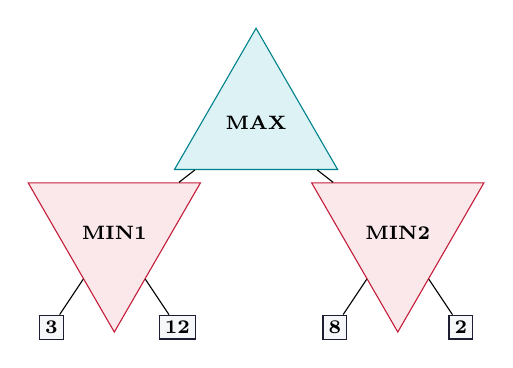
\begin{tikzpicture}[
  level 1/.style={sibling distance=3.6cm, level distance=1.4cm},
  level 2/.style={sibling distance=1.6cm, level distance=1.2cm}
]
  \node [maxnode] {MAX}
    child {node [minnode] {MIN1}
      child {node [leaf] {3}}
      child {node [leaf] {12}}
    }
    child {node [minnode] {MIN2}
      child {node [leaf] {8}}
      child {node [leaf] {2}}
    };
\end{tikzpicture}
\end{tcolorbox}

\subsection{Properties of Minimax}
\begin{itemize}[leftmargin=*, itemsep=3pt]
  \item \textbf{Completeness:} Complete if tree is finite.
  \item \textbf{Optimality:} Optimal against an optimal opponent.
  \item \textbf{Time Complexity:} $O(b^m)$ (explores all tree nodes).
  \item \textbf{Space Complexity:} $O(b \cdot m)$ (depth-first traversal).
\end{itemize}

% ===============================================================================
\section{Alpha-Beta Pruning}
% ===============================================================================

Alpha-Beta pruning removes branches of the game tree that cannot influence the final decision, reducing search time without altering the optimal choice.

\begin{tcolorbox}[defbox, title={Definition of Alpha ($\alpha$) and Beta ($\beta$)}]
  \begin{itemize}[leftmargin=*, noitemsep]
    \item \textbf{$\alpha$ (Alpha):} Highest-value choice found so far along the path for MAX. (Initial value: $-\infty$).
    \item \textbf{$\beta$ (Beta):} Lowest-value choice found so far along the path for MIN. (Initial value: $+\infty$).
  \end{itemize}
\end{tcolorbox}

\begin{tcolorbox}[formulabox, title={Alpha-Beta Pruning Condition}]
  Prune remaining children of node $n$ if:
  \begin{equation}
    \alpha \ge \beta
  \end{equation}
\end{tcolorbox}

\subsection{Effectiveness of Alpha-Beta Pruning}
\begin{itemize}[leftmargin=*, itemsep=3pt]
  \item \textbf{Worst-Case Complexity:} $O(b^m)$ (no pruning occurs if worst moves evaluated first).
  \item \textbf{Optimal Move Ordering Complexity:} $O(b^{m/2})$
  \item With optimal move ordering, Alpha-Beta doubles the solvable search depth!
\end{itemize}

% ===============================================================================
\section{Imperfect Real-Time Decisions}
% ===============================================================================
In real games (Chess, Go), searching to terminal leaves is computationally impossible. We replace terminal tests with \textbf{Cutoff Tests} and terminal utility with \textbf{Evaluation Functions} $Eval(s)$.

\begin{tcolorbox}[examplebox, title={Requirements for Evaluation Functions}]
  \begin{enumerate}[leftmargin=*, noitemsep]
    \item Must rank terminal states in same order as true utility.
    \item Computation must be fast.
    \item Must correlate strongly with win probabilities (e.g., weighted sum of material values in Chess).
  \end{enumerate}
\end{tcolorbox}

\newpage
\begin{center}
  {\large\bfseries\color{myred} Quick Revision --- Module 4}\\[3pt]
  {\small\color{mydark} Adversarial Search \& Game Playing $|$ OE-EC804A}
\end{center}
\noindent{\color{myred}\rule{\linewidth}{1.2pt}}
\vspace{4pt}

\begin{tcolorbox}[formulabox, title={\textbf{Key Concepts and Metrics at a Glance}}]
\renewcommand{\arraystretch}{1.35}
\begin{tabularx}{\linewidth}{B{4.5cm} X}
Minimax Decision & $MAX = \max_{a} Minimax(Result(s,a))$, $MIN = \min_{a} Minimax(Result(s,a))$ \\[4pt]
$\alpha$-$\beta$ Pruning Condition & Prune remaining subtree whenever $\alpha \ge \beta$ \\[4pt]
Optimal Alpha-Beta Time & $O(b^{m/2})$ \quad (Doubles solvable search depth compared to $O(b^m)$) \\[4pt]
Evaluation Function & $Eval(s) = w_1 f_1(s) + w_2 f_2(s) + \dots + w_n f_n(s)$ \quad (Estimates utility at cutoff) \\[4pt]
Zero-Sum Property & $Utility_{MAX}(s) + Utility_{MIN}(s) = 0$ \quad (Constant total utility) \\
\end{tabularx}
\end{tcolorbox}

\begin{tcolorbox}[defbox, title={\textbf{One-Line Definitions}}]
  \begin{itemize}[leftmargin=*, noitemsep]
    \item \textbf{Zero-Sum Game:} Game where total utility across all players sums to zero.
    \item \textbf{Alpha ($\alpha$):} Best (highest) utility value MAX is guaranteed along path.
    \item \textbf{Beta ($\beta$):} Best (lowest) utility value MIN is guaranteed along path.
    \item \textbf{Horizon Effect:} Issue where inevitable bad event is pushed beyond search cutoff depth.
  \end{itemize}
\end{tcolorbox}

\begin{tcolorbox}[exambox, title={\textbf{Frequently Asked / Viva Questions}}]
  \begin{enumerate}[topsep=0pt, label=\textbf{Q\arabic*.}, itemsep=5pt]
    \item \Q{Define a Zero-Sum Game.}
    A game where one player's gain is exactly equal to the other player's loss ($Util_{MAX} + Util_{MIN} = 0$).

    \item \Q{What is the Minimax algorithm?}
    A recursive algorithm for calculating optimal moves in 2-player zero-sum games by maximizing MAX's payoff assuming MIN minimizes it.

    \item \Q{Explain Alpha ($\alpha$) and Beta ($\beta$) parameters.}
    $\alpha$: Best value for MAX found so far. $\beta$: Best value for MIN found so far.

    \item \Q{What is the condition for Alpha-Beta pruning?}
    Branch is pruned when $\alpha \ge \beta$.

    \item \Q{Does Alpha-Beta pruning change the final outcome of Minimax?}
    No, it produces the exact same decision as Minimax while pruning irrelevant branches.

    \item \Q{What is the time complexity of Alpha-Beta with perfect move ordering?}
    $O(b^{m/2})$, which doubles the effective search depth compared to standard Minimax ($O(b^m)$).

    \item \Q{Why are evaluation functions needed in game playing?}
    Because full game trees are too deep to search to terminal states within time limits.

    \item \Q{What is the Horizon Effect?}
    When search depth limit conceals an unavoidable penalty by delaying it past the cutoff.

    \item \Q{Compare Minimax vs Alpha-Beta Pruning.}
    Minimax evaluates all $O(b^m)$ nodes; Alpha-Beta prunes provably suboptimal branches reducing nodes to $O(b^{m/2})$.

    \item \Q{What is Quiescence Search?}
    Search expanded past cutoff depth in non-quiescent (unstable) states to prevent misleading evaluation scores.
  \end{enumerate}
\end{tcolorbox}

\end{document}
